%-------------------------------------------------------------------------------
\section{Motivation}\label{motivation}
%-------------------------------------------------------------------------------

This paper is motivated by the benefits of serverless for workloads like web
applications, and shows that the \problem{} will need to be solved in order to
achieve it.

\subsection{Web applications are a good fit for serverless}

Web applications' traffic patterns make them a great candidate for running as
serverless functions: their load is event-based, bursty and unpredictable, and a
function's resource requirements can vary greatly depending on which user
invoked it.

A back of the envelope calculation shows that for web applications with small
load, lambda functions today are cheaper: with 50K requests per day, a memory
footprint of < 128 MB per function and 200ms of execution, running that on AWS
lambda adds up to \$1.58 per month. On the other hand, the cheapest EC2 instance
costs just over \$3 per month. Of course, as the number of requests goes up, the
price for lambdas scales linearly, whereas running an EC2 instance on full load
becomes comparably cheap. Extensive simulations show a more nuanced picture of
the tradeoff points for different
workloads~\cite{econ-of-serverless,trek10-blog}.

Serverless also may outperform reservation systems for workloads that are very
bursty: starting a new lambda execution environment is much faster than starting
a new container or EC2 instance, which can take multiple
minutes~\cite{ec2-autoscaling}.


\subsection{The \problem{}}


\begin{figure}[t!]
    \centering
      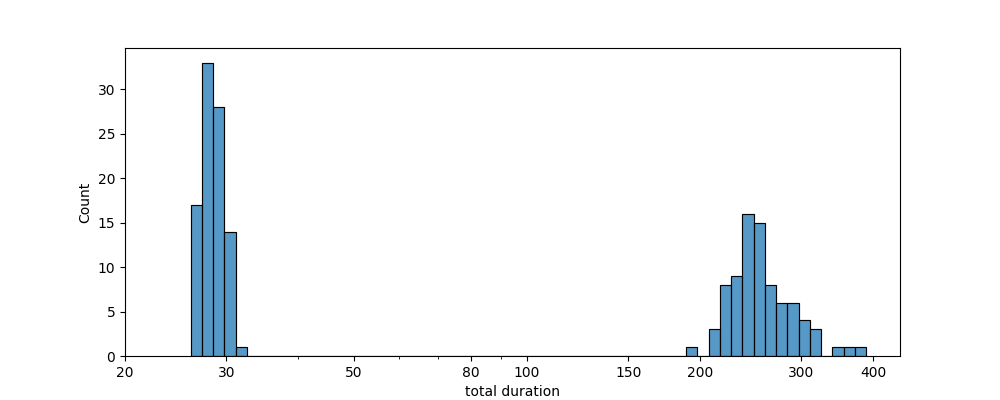
\includegraphics[width=8.5cm]{img/lambda_total_durations.png}
      \caption{ distribution of end to end duration times. The y axis is log scale }
    \label{fig:lambda-total-durations}
\end{figure}


Any system that runs with high average utilization must experience moments where
there is more load than the resources can handle. As we know from recent
traces~\cite{prequal}, although load may look stable at a time increment of
hours or even minutes, going down to the second level shows the load to have
high variance. If providers want to have good average utilization, then in the
moments of load spike the load will be more than the resources can handle.

In a multi tenant setting, what this means is that one developers exprienced
latencies will depend on other people's load. This is not ideal, expecially if
one developer's user facing function is queued while another developers
background task is running. This situation is the essence of the \problem{}.

We can see evidence of the \problem{} occurring in lambda invocations today,
within the cold start invocations. We run an experiment with a simple lambda
function that sleeps for 20ms and then returns. We use AWS Xray~\cite{aws-xray}
to measure its latency, with incovations spaced randomly between 0 and 10
minutes. The results are in Figure~\ref{fig:lambda-total-durations}. The spike
on the left side of the graph is the execution times from invocations that used
warm start. The durations remain stable, because AWS is able to simply route the
new request to the machine with the existing container. We verify this what is
happening by changing the function to include reading and then writing to an
environment variable, and find that for invocations with warm start when we read
the variable it was already set by a previous invocation.

The right grouping in the graph is those invocations that hit cold starts, whose
overall latencies vary between $\sim$200 and $\sim$400ms. This variance
indicates that there is something more going on than just waiting for a
container to start.

Although AWS' scheduling mechanism is proprietary, we can look to open source
alternatives to see what common best practices exist today. Schedulers have two
different options when load exceeds compute capacity: queue the excess load, or
place it on machines and let them deal with being temporarily overloaded.
Different schedulers have different approaches. 

In OpenWhisk~\cite{openwhisk}, the load balancer will choose which machine to
run the function on, and then place the invocation, adressed to that machine,
into a Kafka queue that the machine subscribes to and can pull the invocation
from when it is ready~\cite{openwhisk-sched}. This means that in the case of
high load, a latency sensitive function might sit in the Kafka queue while
someone else's background function completes: the \problem{}. 

Knative~\cite{knative} similarly queues the excess invocations, although it does
so via the load balancer, which is also in charge of
autoscaling~\cite{knative-sched}: if the existing pods are fully loaded (with a
small, bounded-size queue in front of them), requests are queued separately
while the autoscaler starts up more invocations. Again, latency sensitive
functions are potentially waiting for someone else's background function
completes: the \problem{}. 

Hermod~\cite{hermod} is a recent research serverless scheduler, and shows in a
simulation that late binding (as openwhisk and knative do) performs worse than
early binding. Under high load, Hermod places the excess functions on machines
anyway (used a least loaded policy) and does Processor Sharing scheduling among
them. This ensures that no one function has a high delay, but rather that all
are equally slowed down. This still leads to the \problem{} though, just that
now rather than experiencing queueing the latency senstive function is
experiencing delay. The paper also does not address what happens when the
machines are out of memory. 

Because none of these schedulers have information about the functions they are
queueing, it is impossible for them to know which to prioritize. The way all of
the above schedulers avoid the \problem{} is by doing different forms of
accounting concurrency: concurrency can be reserved or provisioned for specific
functions, and limited for others. This is necessary to ensure that a burst in
background tasks doesn't starve the latency sensitive functions. However, what
happens when the datacenter is out of resources and so the concurrency limit has
not yet been reached but the resources are unavailable is not clear. Reserving
and provisioning and limiting are also conceptually in tension with the goal of
serverless, which is to be on-demand and flexible.



% It is impossible to know what proprietary systems like AWS do, but since AWS
% guarantees an amount of memory as well as a fraction of vCPUs to each function,
% it is likely AWS also queues the invocations to ensure they aren't put in a
% position of having to break those guarantees.\hmng{that might be a test we could
% run: do a tight while loop and look at cpu time and wall clock time to see how
% we are being scheduled} 


